% meta.concepts: 3D force equilibrium
% meta.tags: realistic
% acknowledge: Engineering Statics: Open and Interactive
% source: Example  3.5.3 of January 10, 2023 edition

A hot air balloon $30 ft$ above the ground is tethered by three cables as shown in the diagram. If the balloon is pulling upwards with a force of $900 lb$, what is the tension in each of the three cables? The grid lines on the ground plane are spaced $10 ft$ apart.

\begin{figure}[ht!]
  \centering
  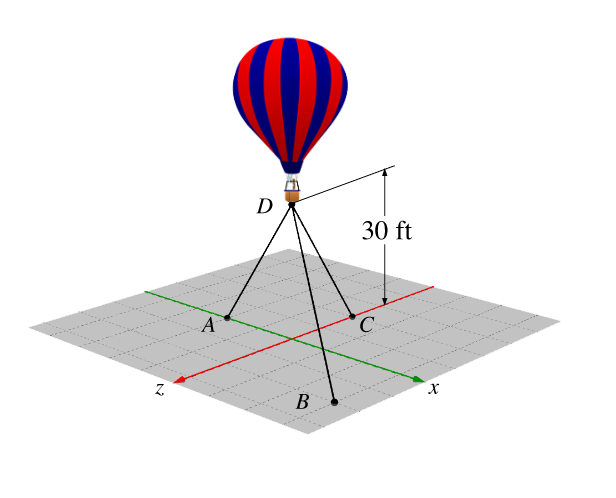
\includegraphics[width=0.8\textwidth,height=0.4\textheight,keepaspectratio]{fig.png}
\end{figure}

\iftoggle{flagSoln}{%
\vspace{.5cm}
\rule{\textwidth}{.4pt}
\vspace{.5cm}
\textbf{Solution:}
\begin{figure}[ht!]
  \centering
  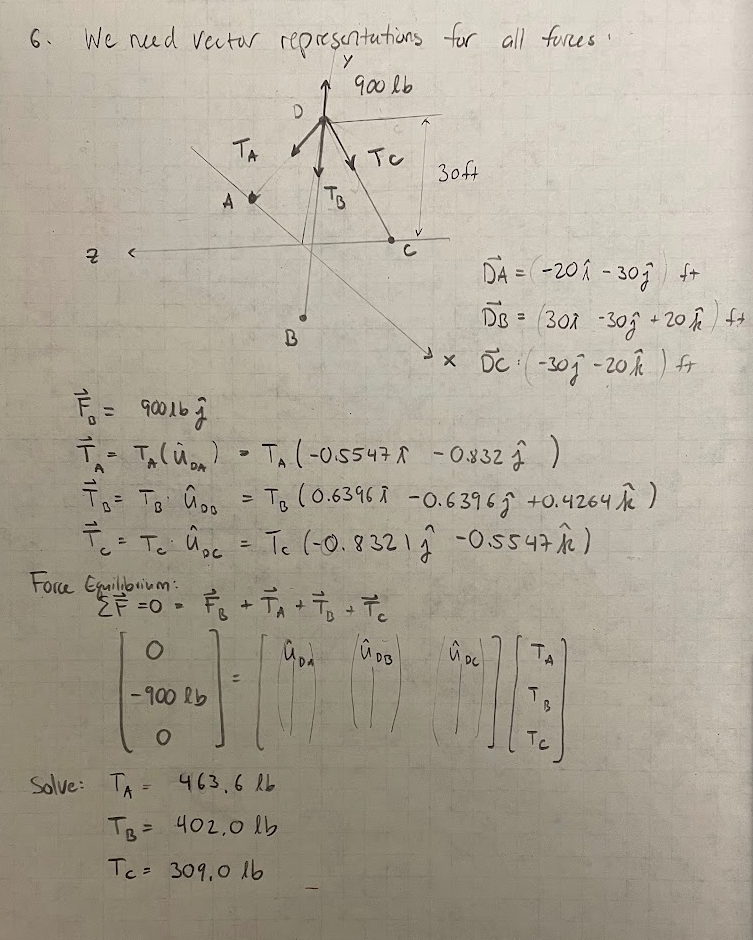
\includegraphics[width=0.9\textwidth,
	           height=0.4\textheight,
		   keepaspectratio]{soln.png}
\end{figure}
}{%
}%
